\documentclass[12pt,a4paper,twoside]{ctexart}

%\usepackage{ctex}
%\usepackage{xeCJK}
\usepackage[utf8]{inputenc}


\usepackage{amsmath,amsthm,amssymb, slashed,upgreek,url,graphicx}

\usepackage[bookmarks=true,colorlinks,citecolor=black,linkcolor=black]{hyperref}
\usepackage{float}
\usepackage[svgnames]{xcolor}
\usepackage{subfig}
\usepackage{mathtools,nccmath}

\usepackage{fontspec}
\setCJKmainfont{FandolSong-Regular}[ BoldFont = FandolSong-Bold , ItalicFont = FandolKai-Regular ]



\numberwithin{figure}{section}

\numberwithin{equation}{section} 


\usepackage{listings}

\usepackage{fancyhdr}%页眉页脚宏包



\usepackage{geometry}%页面宏包
\geometry{a4paper,left=25mm,right=20mm,top=25mm,bottom=20mm}%设定页面
\pagestyle{fancy}%fancy 在geometry 后面
\fancyhf{}
\renewcommand{\headrulewidth}{0.15mm}%页眉线大小
\fancyhead[C]{作业报告}
\fancyfoot[RO,LE]{\thepage}
\setlength{\headheight}{15pt}
\linespread{1.5} %设定行距


\renewcommand{\contentsname}{目录} % default is {Contents}




\pagenumbering{Roman}

\title{{\bf\Huge 孔明棋 Peg Solitaire}\\ \normalsize 作业报告}
\date{2024 年 6 月 20 日}

\lstset{
    language=C++, % 设置语言
    basicstyle=\zihao{-5}\ttfamily, % 设置字体族
    breaklines=true, % 自动换行
    keywordstyle=\bfseries\color{magenta}, % 设置关键字为粗体,颜色
    morekeywords={IMAGE}, % 设置更多的关键字,用逗号分隔
    emph={cleardevice, loadimage, putimage, AlphaBlend, FlushBatchDraw, putimage_alpha, BeginBatchDraw, initgraph}, % 指定强调词,如果有多个,用逗号隔开
    emphstyle=\bfseries\color{NavyBlue}, % 强调词样式设置
    commentstyle=\color{Green!90!black}, % 设置注释样式,斜体,浅灰色
    stringstyle=\bfseries\color{black!50!white}, % 设置字符串样式
    columns=fixed,  % 如果不加这一句,字间距就不固定,很丑,必须加
    basewidth=0.5em,
    numbers=left, % 显示行号在左边
    numberstyle=\zihao{-5}\ttfamily, % 缩小行号
    frame=lrtb, % 边框
}



\begin{document}
\maketitle
\setcounter{page}{0}
\thispagestyle{empty}

\newpage

\tableofcontents%目录


\newpage
\pagenumbering{arabic}

\section{概览}
\subsection{功能描述}
游戏界面如下,点 PLAY 键开始游戏。点左上角按钮退回菜单。点右上角按钮悔棋。
\begin{figure}[ht]
    \centering
    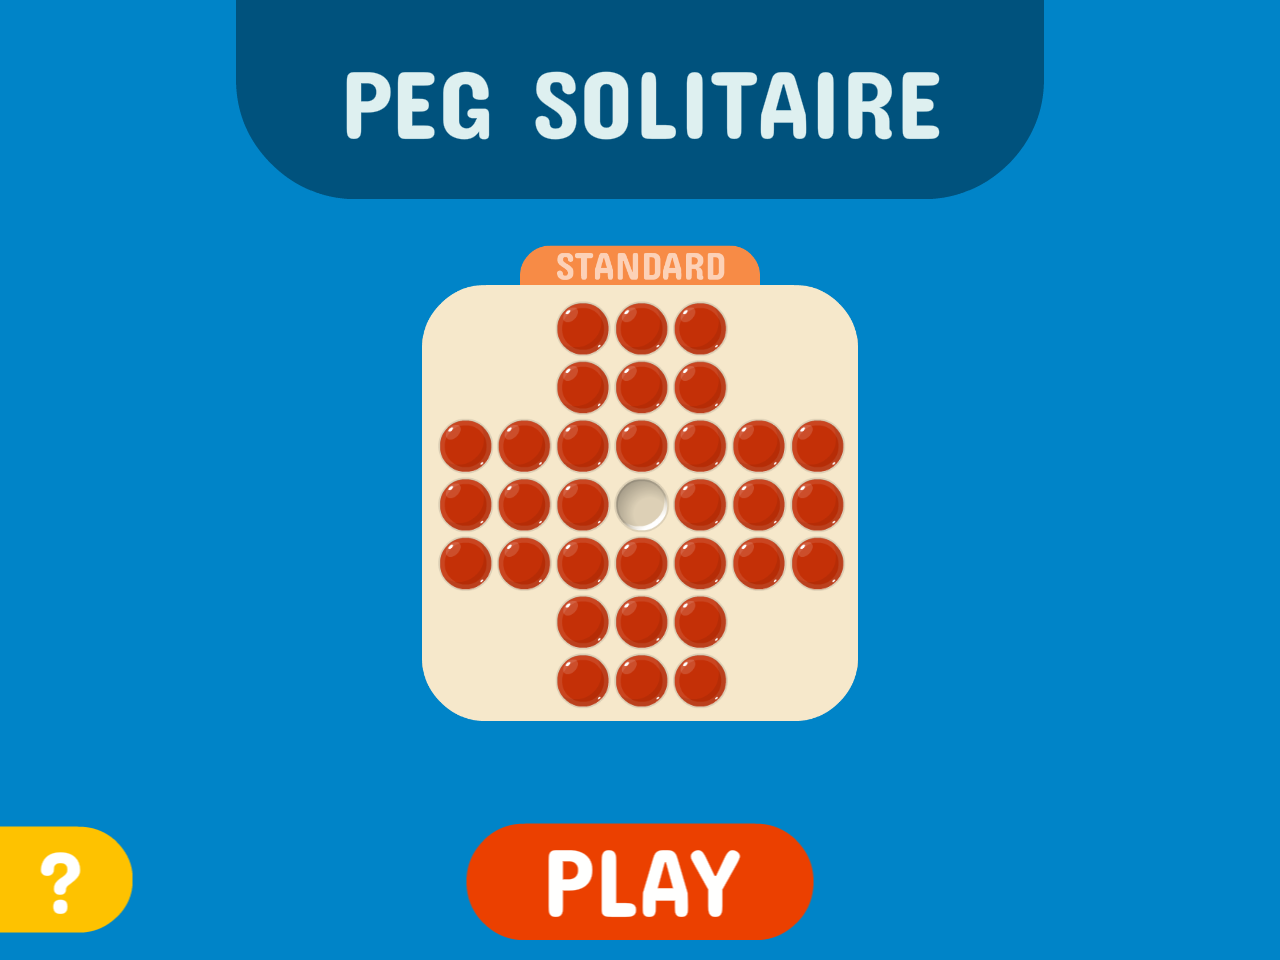
\includegraphics[width=.45\textwidth]{background.png}
    \quad
    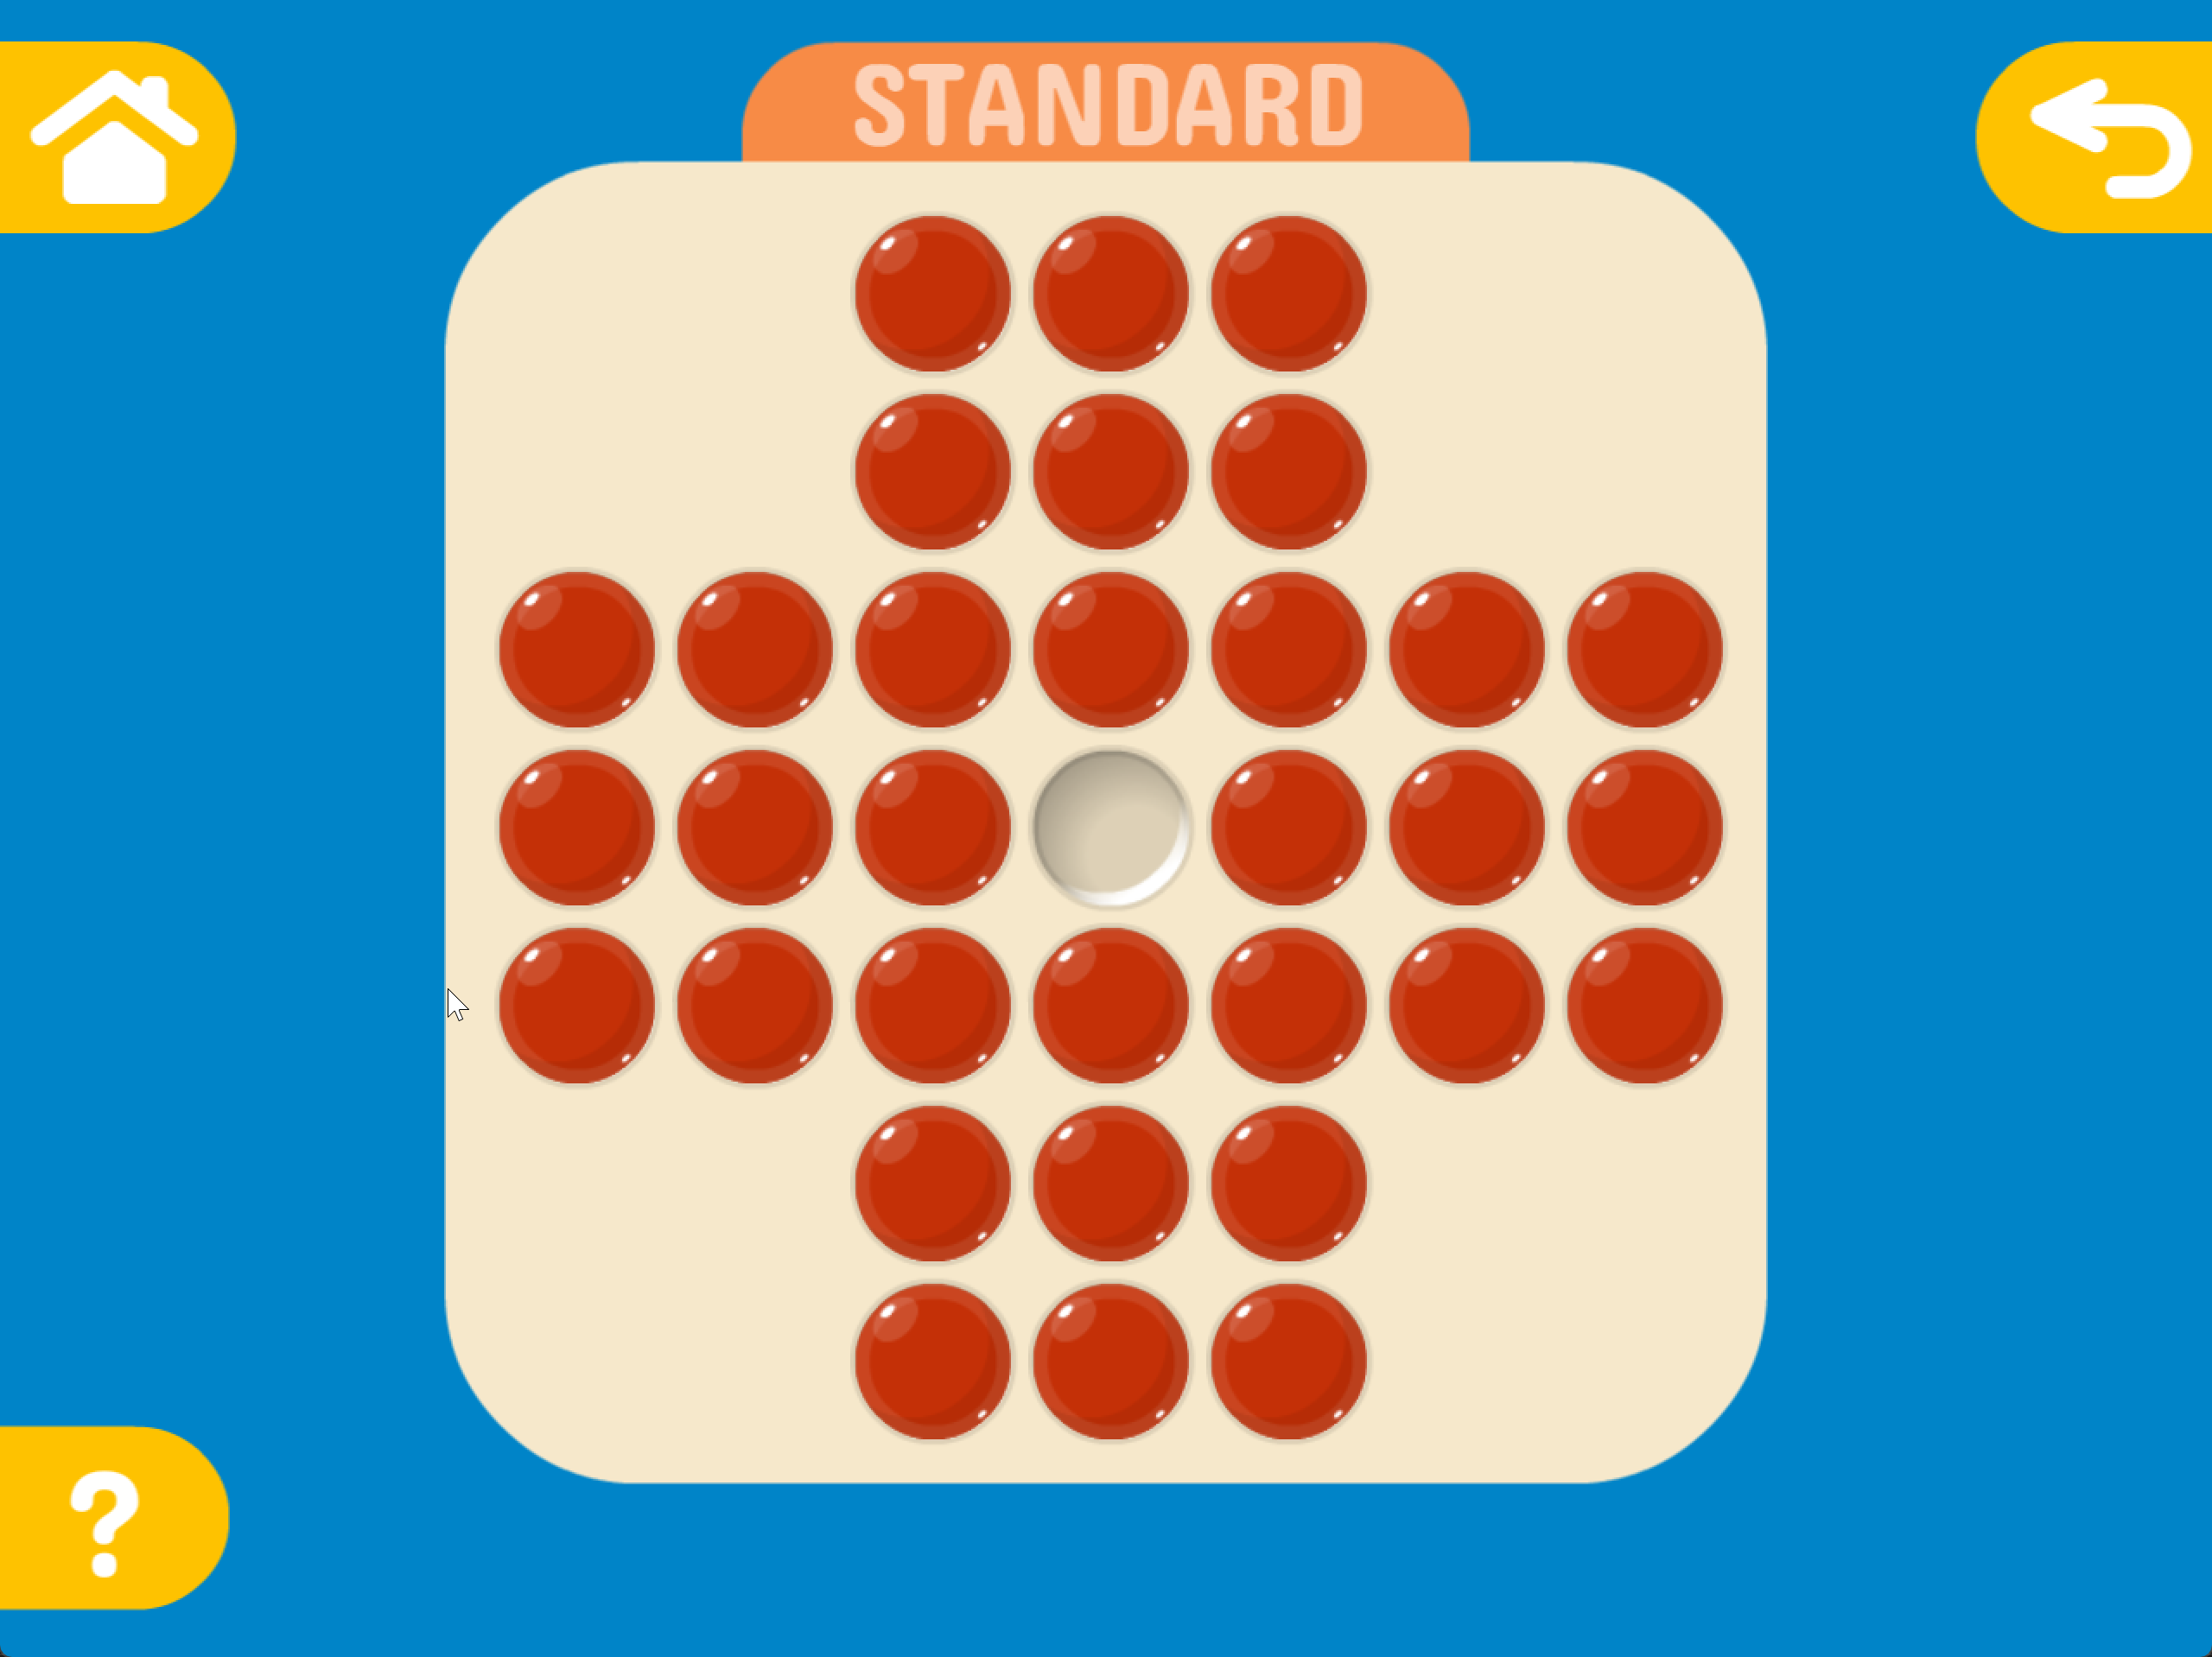
\includegraphics[width=.45\textwidth]{standard.png}
    \caption{菜单和标准棋盘}
\end{figure}

点击左下角按钮可显示帮助。点 OK 键退出。
\begin{figure}[ht]
    \centering
    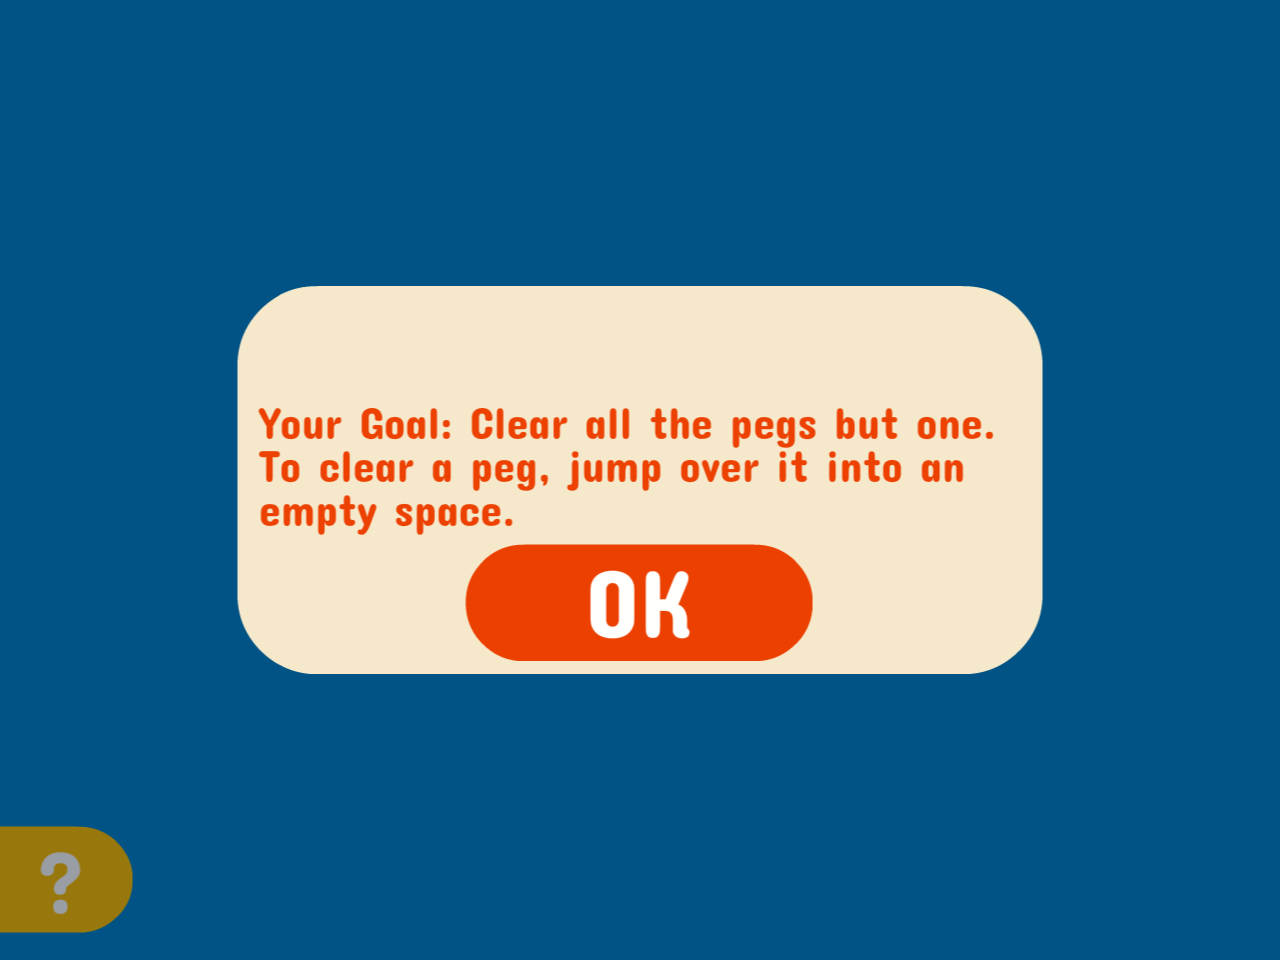
\includegraphics[width=.45\textwidth]{help.png}
    \caption{帮助}
\end{figure}



残局模式通过隐藏按键(1, 2, 3, 4)进入,比如,可按 1 进入心形局.
\begin{figure}[ht]
    \centering
    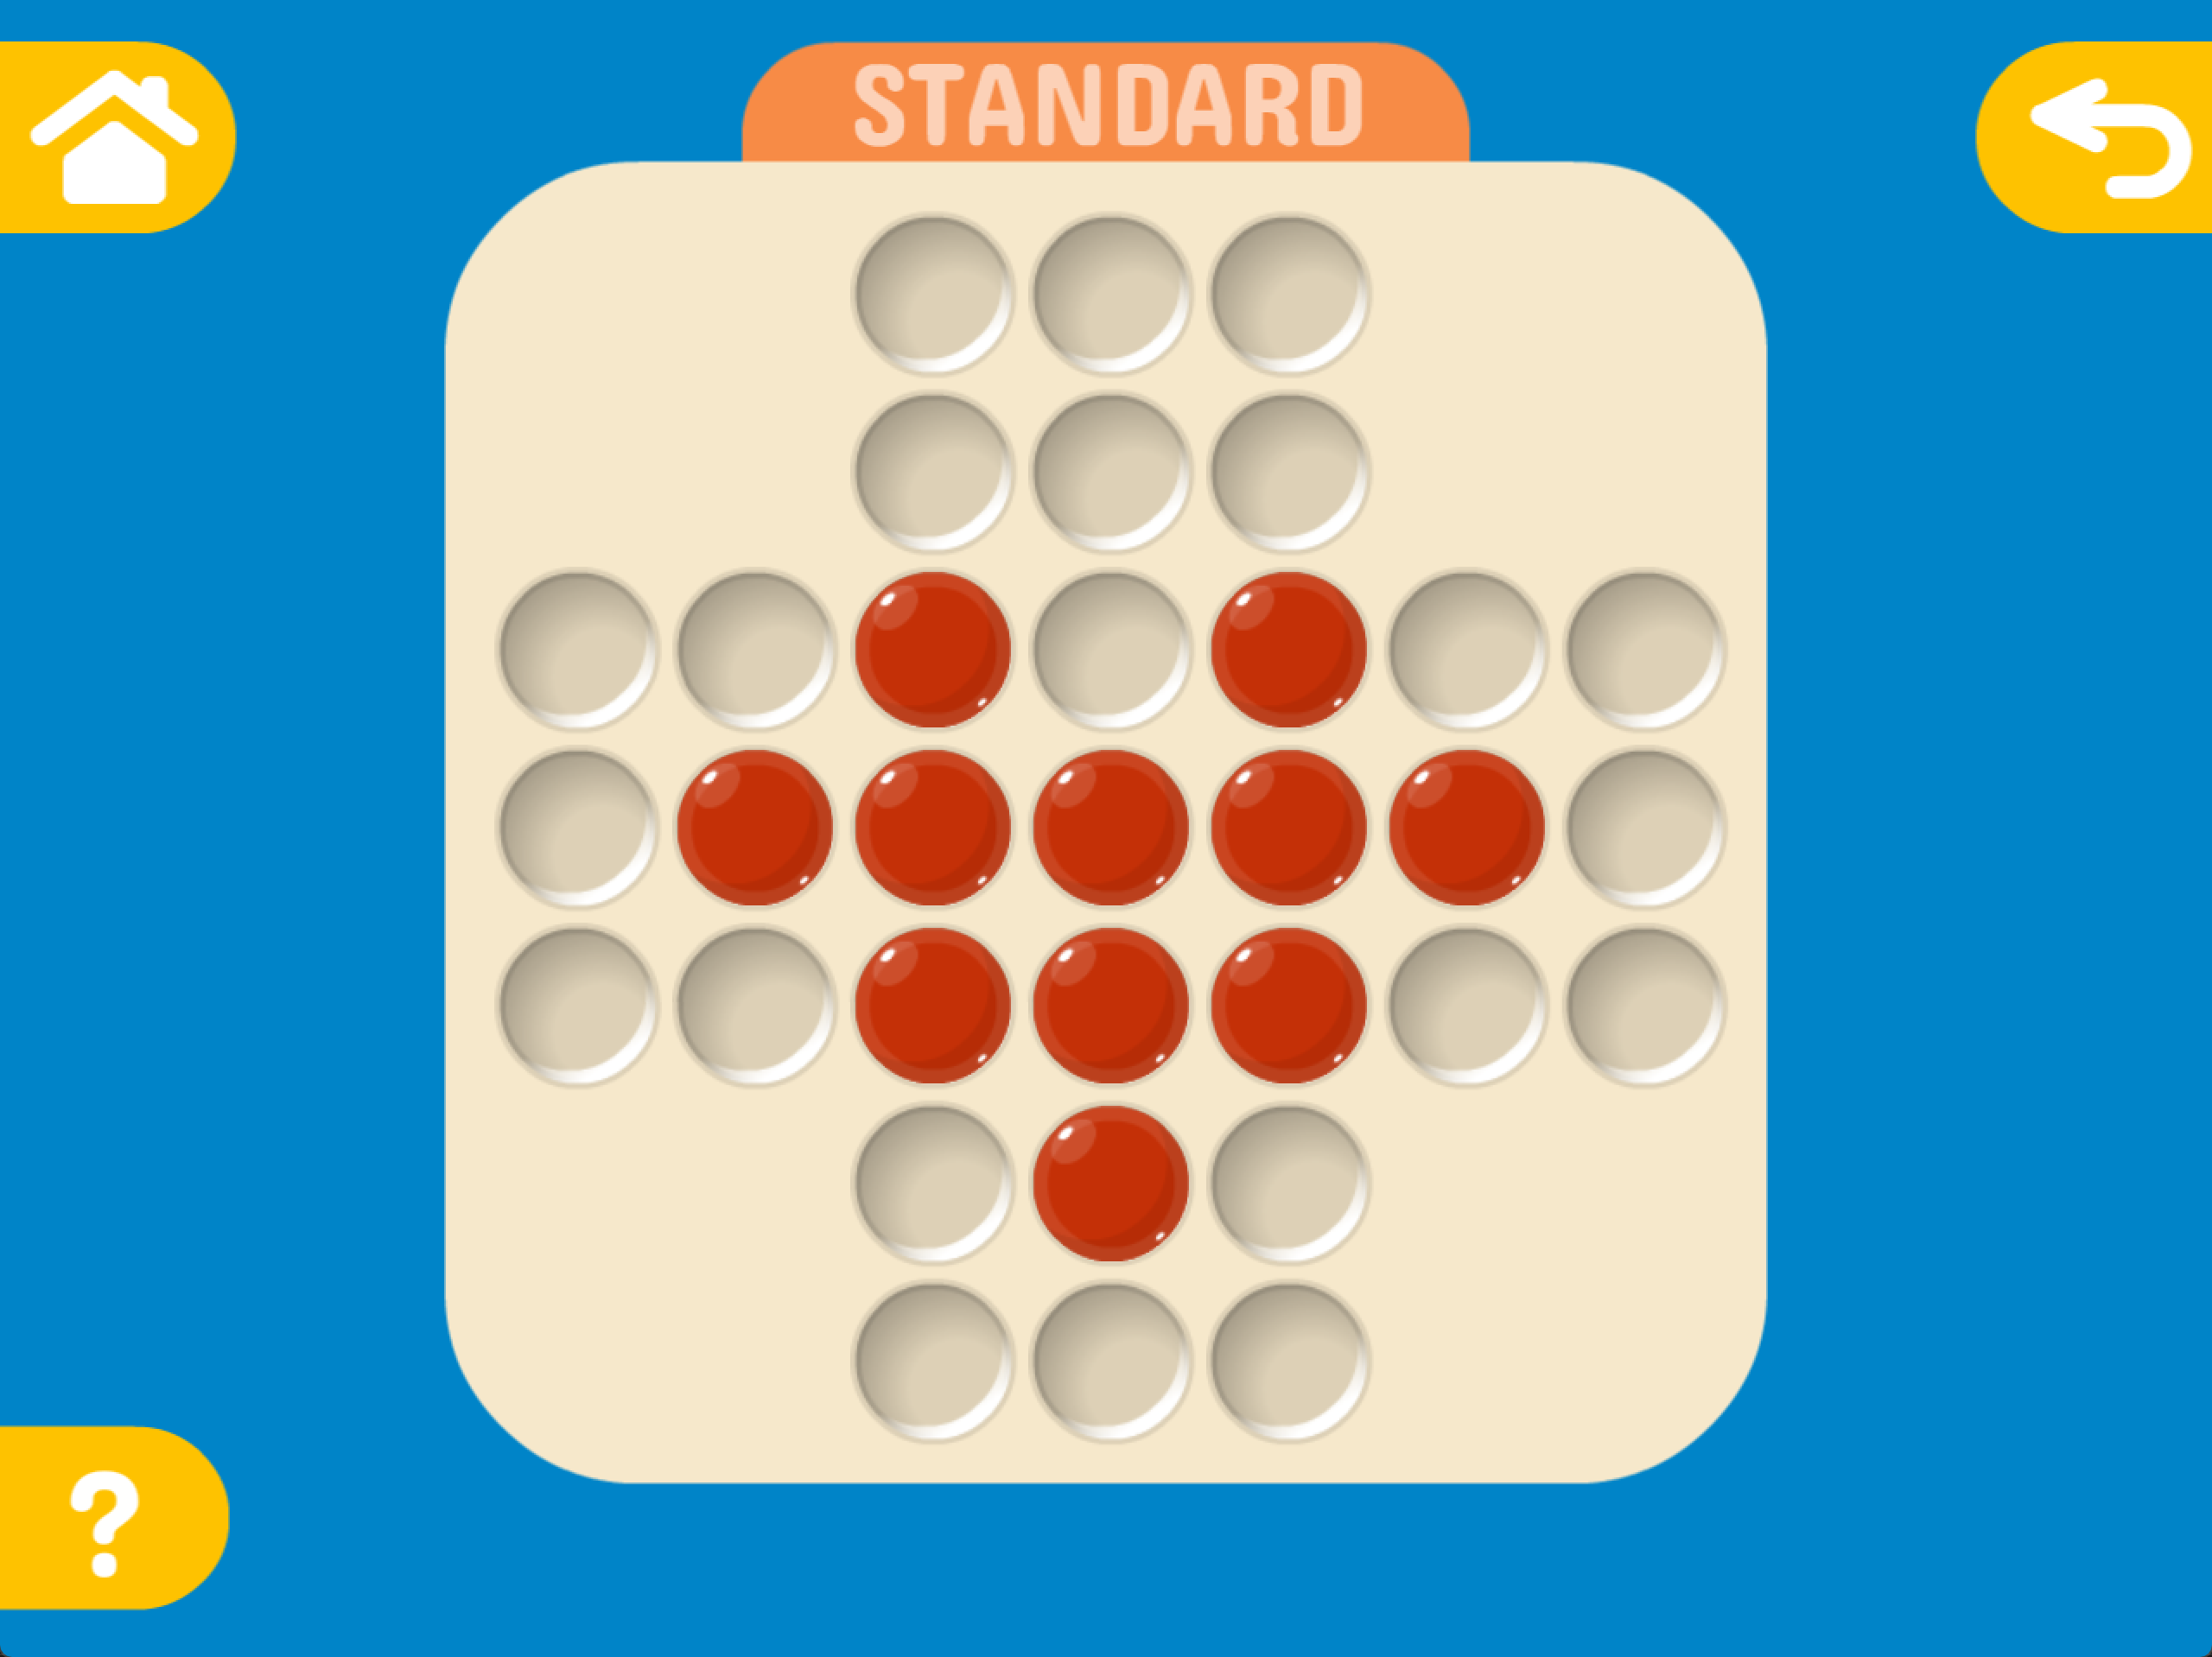
\includegraphics[width=.45\textwidth]{heart.png}
    \caption{心形残局}
\end{figure}

无子可落时代表游戏结束。在此基础上若仅剩一子,则游戏胜利。
\begin{figure}[ht]
    \centering
    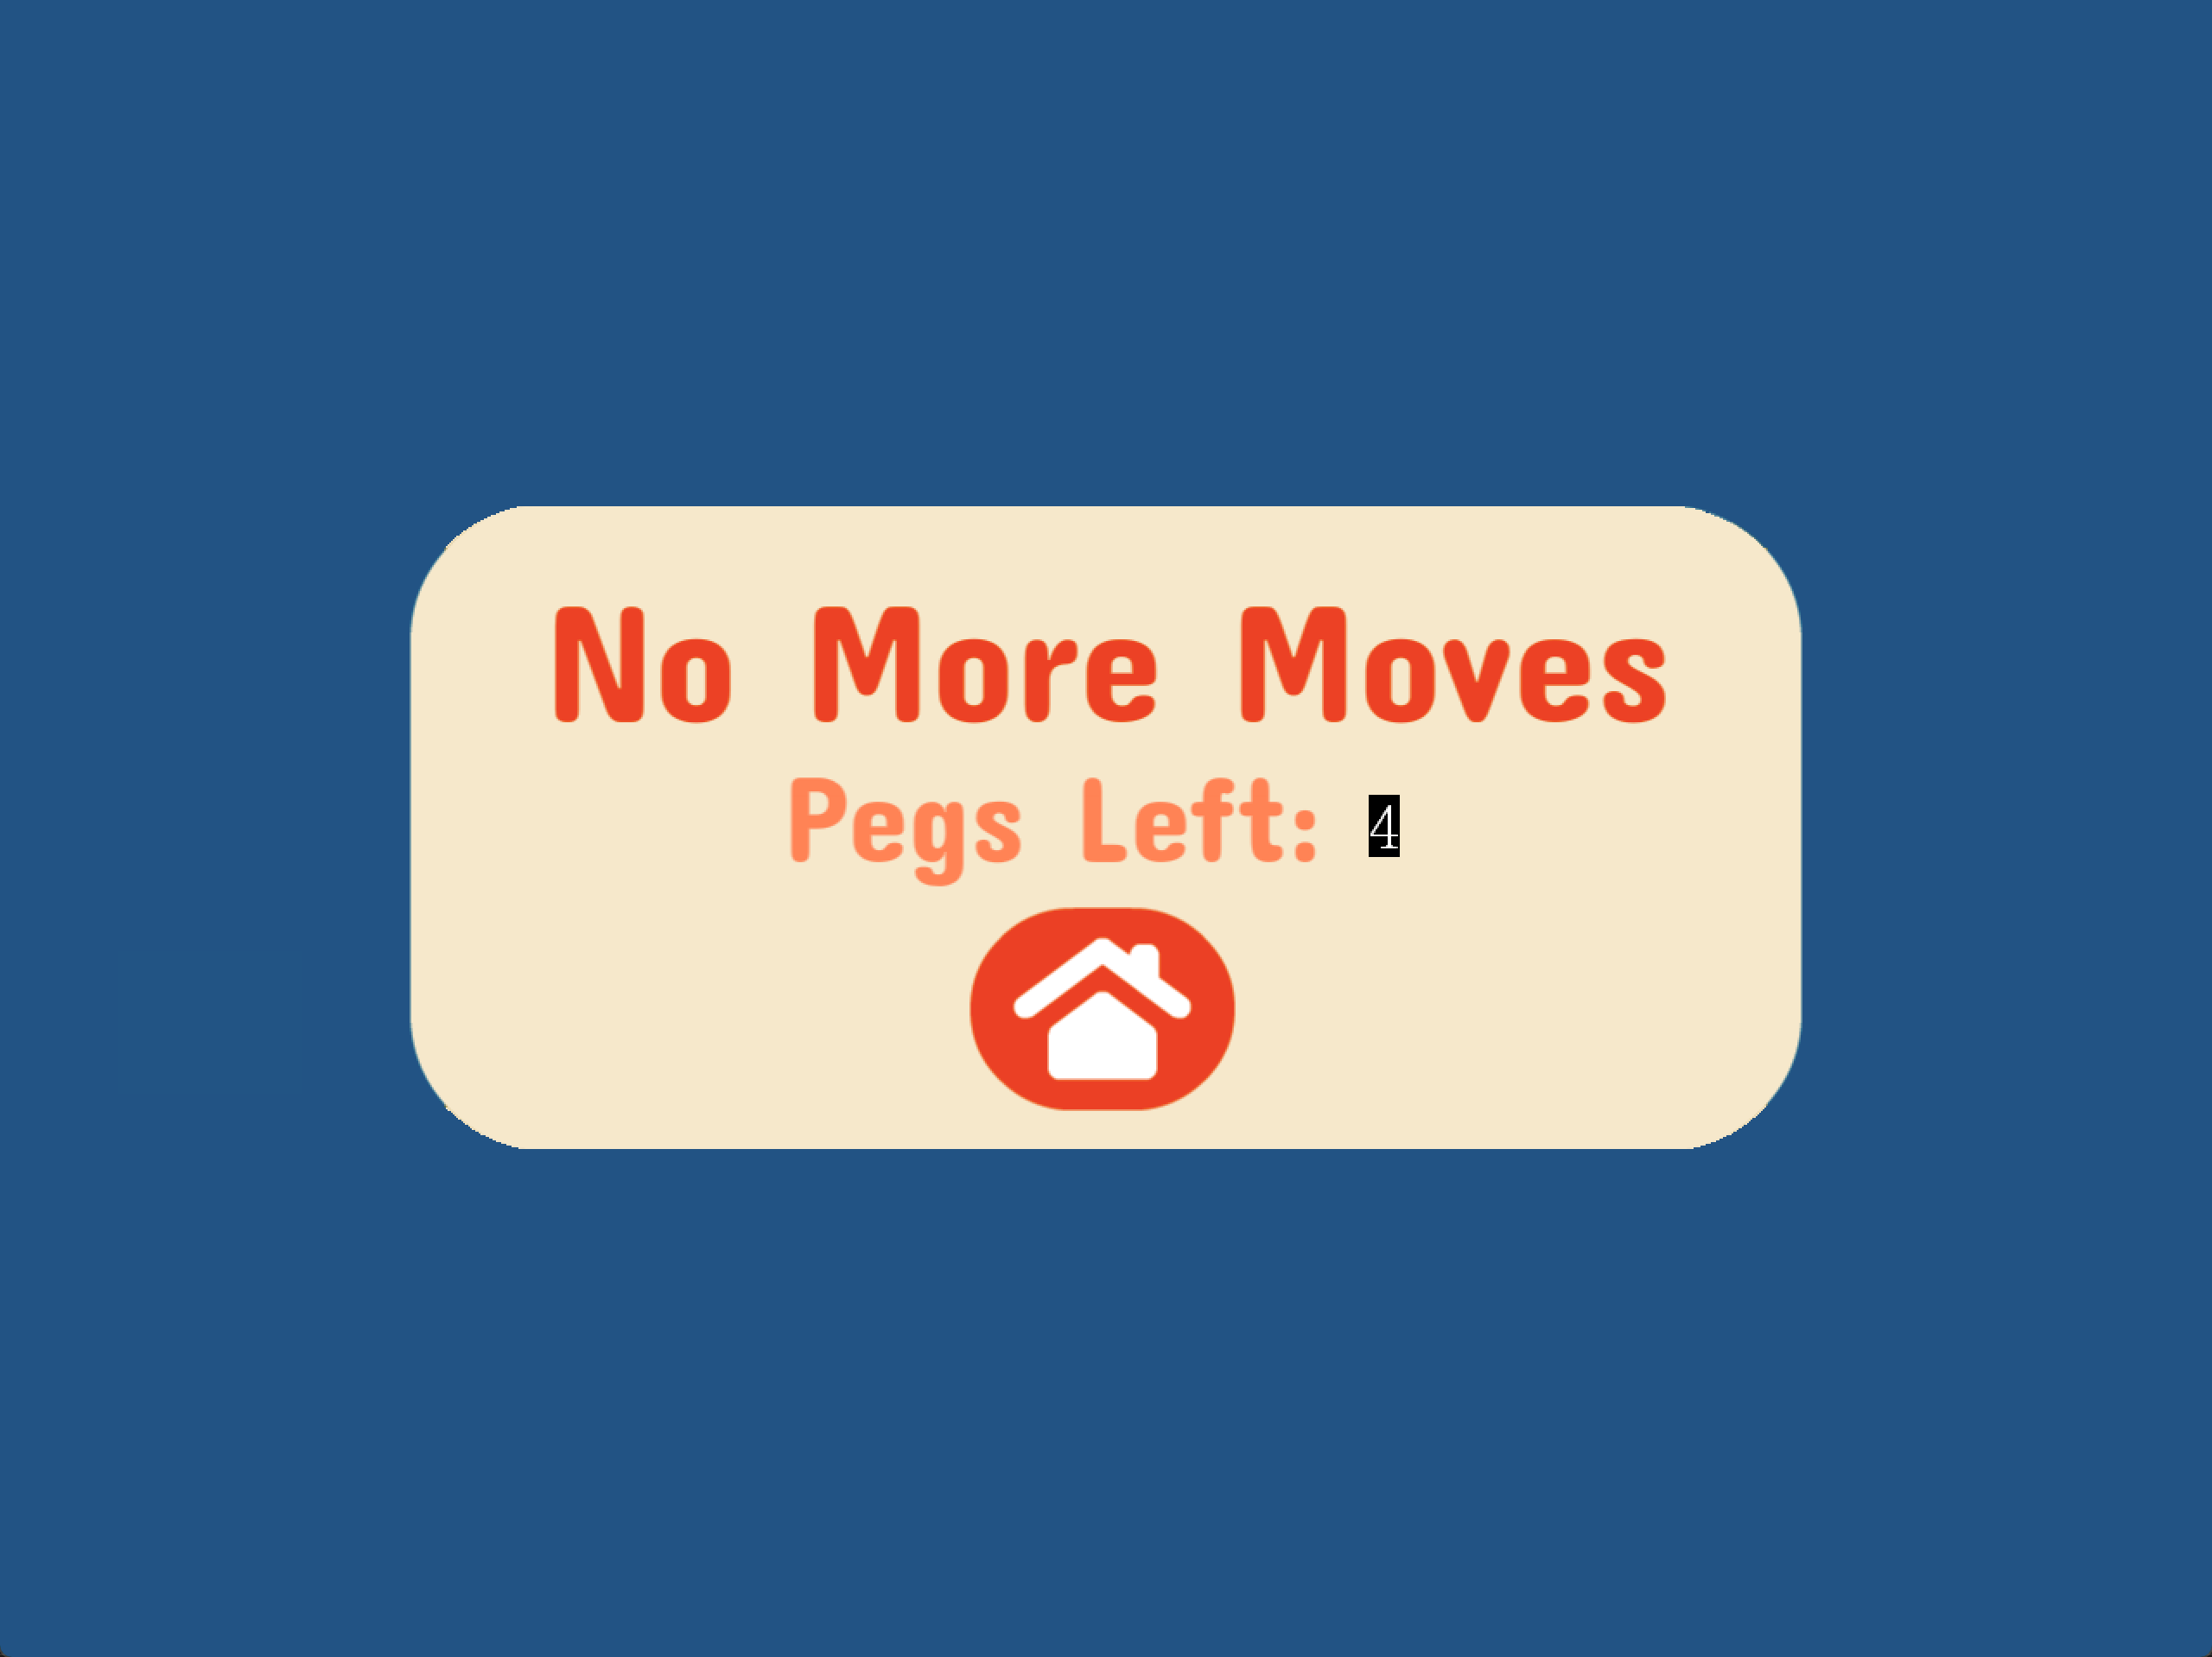
\includegraphics[width=.45\textwidth]{end.png}
    \quad
    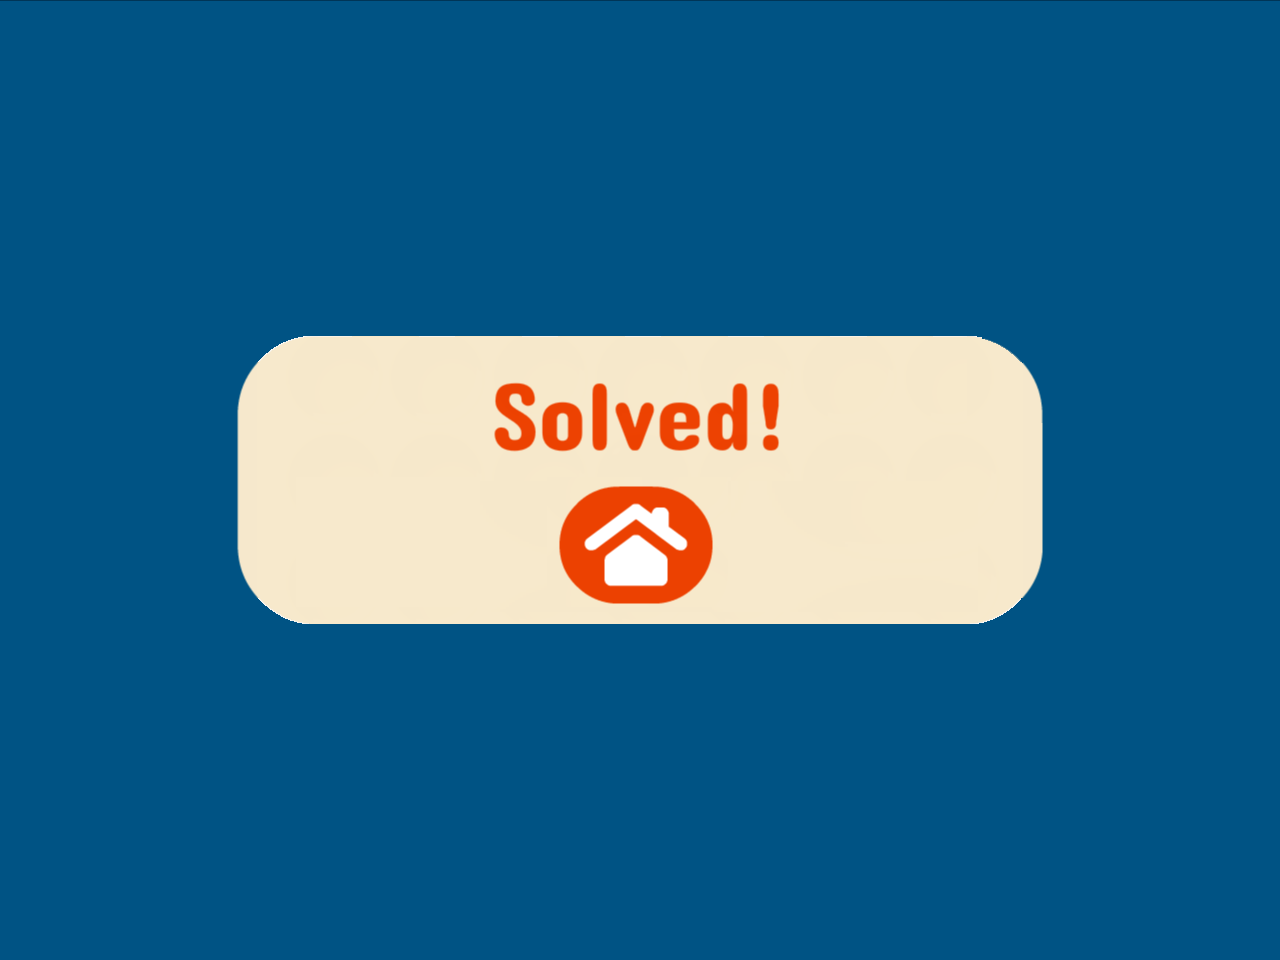
\includegraphics[width=.45\textwidth]{solved.png}
    \caption{普通结束和胜利画面}
\end{figure}

\subsection{设计思路}
主要考虑使用 EasyX 图形库设计游戏。easyX 的基本函数(图形库结合 Windows API)包括加载图片 \verb|loadimage|、在某坐标插入图片 \verb|putimage| 和一些其它的缓冲函数(防止闪烁)。

用户交互通过鼠标,鼠标信息记录为 \verb|ExMessage mouse_msg|,其获取函数为 \verb|getmessage|。基本逻辑是通过鼠标指针的位置以及按键信息,判断用户的操作。

游戏的基本逻辑是用数组存储棋盘和空位信息。有时棋盘并非完整的方形,故聪明的做法是将那些非棋盘区域设置为 \verb|-1|。用类 \verb|class standard| 单独存储各种变量:棋盘、悔棋记忆、剩余数量、玩家选择、玩家落点,以及函数:显示空棋盘、显示当前棋子布局、显示选择状态(和周围可走空位)、游戏结束判断。除此之外,可加上棋子移动的动画效果。这些功能在游戏主循环函数中的实现是一目了然的。

动画设计上的细节是,不仅可以使棋子滑到终点,还可使其大小先增大后减小以模拟一种飞跃感;同时,所消去的棋子也可用一个大小的连续变化来过渡,而非直接消失。

\begin{figure}[ht]
    \centering
    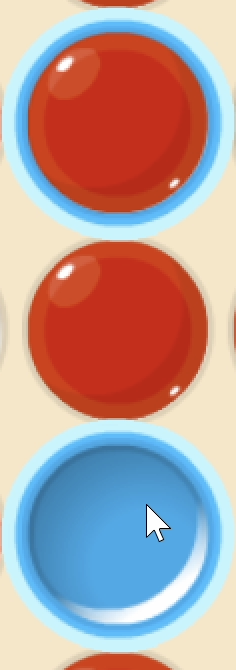
\includegraphics[width=.1\textwidth]{1.png}
    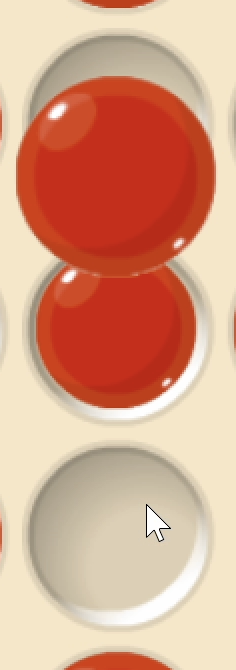
\includegraphics[width=.1\textwidth]{2.png}
    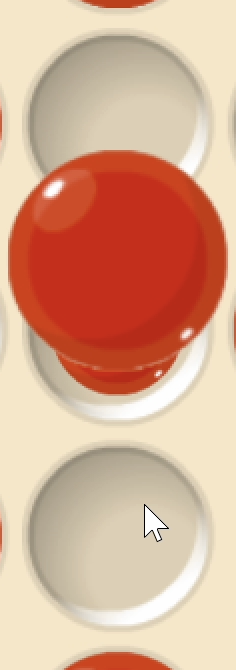
\includegraphics[width=.1\textwidth]{3.png}
    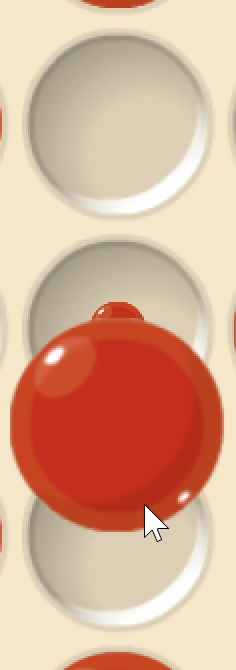
\includegraphics[width=.1\textwidth]{4.png}
    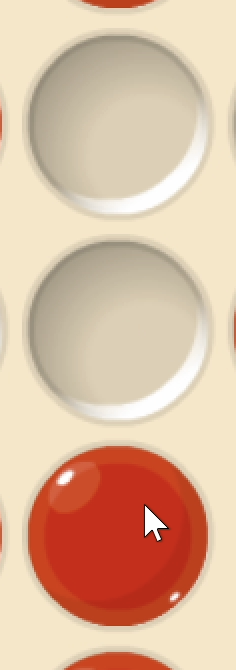
\includegraphics[width=.1\textwidth]{5.png}
    \caption{飞跃过程的 5 次截取。实际帧数为 20,可设置}
\end{figure}

残局模式使用的棋盘仍然是标准棋盘,只是布局上棋子并非 32 颗。因此,只需用一个结构体 \verb|struct other_standard| 存储这些残局情况即可。在实际游戏中,根据玩家所按下的隐藏按键,调用相应棋子布局并进行替换。

对于三角排列的棋盘,数组设置仍然基于方形原则,只是在显示时错位,且一个棋子要考虑的是周围六个方向上的情况(本行是左右两颗,上行则是与本棋相邻两颗,下方同理)。其余的游戏逻辑有大量地方需要从方形情形修改,因此要用另一个类存储。 此外,AI 破解棋局的基础是遍历,但在优化上需要借助路径记忆防止栈溢出。这些功能由于时间因素未完善,但原则上实现逻辑仍然是通俗的。



\newpage
\section{问题及解决方法}
\subsection{素材}
需要花许多时间使用 PS 抠图。比如有如下棋子素材。

\begin{figure}[ht]
    \centering
    
\includegraphics[width=.1\textwidth]{piece.png}
    \quad
    
\includegraphics[width=.1\textwidth]
    {piece_moveTo.png}
    \quad
    
\includegraphics[width=.1\textwidth]
    {piece_resized.png}
    \caption{棋子状态}
\end{figure}

\subsection{音效}
库和函数都准备好,且音效素材也准备好为 wav 形式,可于项目文件中查看。但在音效播放上出现了未知问题,可能与 AU 剪辑导出音频的设置有关。

\subsection{动画}
动画实现飞跃时,大小可通过二次函数 \verb|size = a * (n - step) * n| 形式来构造,其中 \verb|step| 表示动画帧数,而函数的其它项根据实际需求确定,比如可加上棋子边长作为常数项。

\subsection{透明显示}
显示透明颜色需要图像的 alpha 通道,编写一个专门的函数。可见后文。

\newpage
\section{心得体会}

\subsection{算法设计}
主要算法并没有困扰我太多。甚至,由于这次游戏逻辑比较简单,可以脱离 AI 帮助。只是需要花时间查找关于 EasyX 的资料。


\subsection{对结构体和类的理解}
结构体相较于数组的优势在于其可以存储不同类型的数据,且调用语法更直观。而类在此基础上还支持公私之分,可用于将其对应的函数封装起来,可供外界随时调用。当然,底层变量则封锁起来。

\subsection{游戏攻略}
据说可以采取一种螺旋式的走棋方向。

\subsection{所思所想}
为了实现前端,工作量实在太肝,包括抠图、动画制作、坐标 debug,甚至还有则此没有实现的颜色深浅控制。然而结果却又比较赏心悦目,这何尝不是一种补偿性自虐。

\newpage
\section{部分源代码}

\begin{lstlisting}[
    caption     =   {透明显示},
]
inline void putimage_alpha(int x, int y, IMAGE* img) {
	int w = img->getwidth();
	int h = img->getheight();
	AlphaBlend(GetImageHDC(NULL), x, y, w, h,
		GetImageHDC(img), 0, 0, w, h, { AC_SRC_OVER,0,255,AC_SRC_ALPHA });
}
\end{lstlisting}

\begin{lstlisting}[
    caption     =   {飞跃动画},
]
void move_animation(int x, int y, int to_x, int to_y, int step) {
    for (int n = 0; n < step; ++n) {
        show_board();
        show_pieces();

        float fading_size = 0.1 * n * (step - n) + 92 - (92 * n / step);
        IMAGE fading_piece;
        loadimage(&fading_piece, _T("image/piece.png"), fading_size, fading_size);
        putimage_alpha(x + (to_x - x) / 2 - (fading_size - 92) / 2, y + (to_y - y) / 2 - (fading_size - 92) / 2, &fading_piece);

        float flying_size = 0.4 * n * (step - n) + 92;
        IMAGE flying_piece;
        loadimage(&flying_piece, _T("image/piece.png"), flying_size, flying_size);
        putimage_alpha(x + n * (to_x - x) / step - (flying_size - 92) / 2, y + n * (to_y - y) / step - (flying_size - 92) / 2, &flying_piece);
        FlushBatchDraw();
    }
}
\end{lstlisting}

动画函数存储在类 \verb|class Game game| 里。

然后是一些游戏的主干架构,同样存储在类中。本程序的结构体用于存储棋盘数据。

\begin{lstlisting}[
    caption     =   {游戏主循环},
]
void game() {
	save_memory();
	while (1) {
		show_board();
		show_pieces();

		getmessage(&mouse_msg);

		//通过隐藏按键进入残局
		if (mouse_msg.message == WM_KEYDOWN) {
			if (mouse_msg.vkcode == '1') {
				remaining = 11;
				for (int i = 0; i < 7; ++i) {
					for (int j = 0; j < 7; ++j) {
						board[i][j] = canju.board_1[i][j];
					}
				}
			}
			if (mouse_msg.vkcode == '2') {
				remaining = 8;
				for (int i = 0; i < 7; ++i) {
					for (int j = 0; j < 7; ++j) {
						board[i][j] = canju.board_2[i][j];
					}
				}
			}
			if (mouse_msg.vkcode == '3') {
				remaining = 8;
				for (int i = 0; i < 7; ++i) {
					for (int j = 0; j < 7; ++j) {
						board[i][j] = canju.board_3[i][j];
					}
				}
			}
			if (mouse_msg.vkcode == '4') {
				remaining = 6;
				for (int i = 0; i < 7; ++i) {
					for (int j = 0; j < 7; ++j) {
						board[i][j] = canju.board_4[i][j];
					}
				}
			}
		}

		if (mouse_msg.message == WM_LBUTTONDOWN) {
			//悔棋
			if (mouse_msg.x >= 1143 && mouse_msg.x <= 1280 && mouse_msg.y >= 25 && mouse_msg.y <= 156) {
				if (memory_count > 0) {
					memory_count--;
					for (int i = 0; i < 7; ++i) {
						for (int j = 0; j < 7; ++j) {
							board[i][j] = memory[i][j][memory_count];
						}
					}
				}
				X = Y = to_X = to_Y = -1; //不显示
			}
			//退出
			else if (mouse_msg.x >= 0 && mouse_msg.x <= 137 && mouse_msg.y >= 25 && mouse_msg.y <= 156) break;

			//棋盘内
			if (mouse_msg.x >= 288 && mouse_msg.x <= 288 + 7 * 103 && mouse_msg.y >= 125 && mouse_msg.y <= 125 + 7 * 103) {
				int state = board[(mouse_msg.y - 125) / 103][(mouse_msg.x - 288) / 103]; //此处状态
				//棋子
				if (state == 1) {
					X = (mouse_msg.x - 288) / 103;
					Y = (mouse_msg.y - 125) / 103;
				}
				//空位
				else if (state == 0) {
					to_X = (mouse_msg.x - 288) / 103;
					to_Y = (mouse_msg.y - 125) / 103;
				}
			}
			//帮助
			else if (mouse_msg.x >= 0 && mouse_msg.x <= 131 && mouse_msg.y >= 824 && mouse_msg.y <= 939) {
				help();
			}
		}

		show_selected(); //显示选中棋子&可走空位

		if (can_move()) {
			remaining--;
			move_animation(288 + X * 103, 125 + Y * 103, 288 + to_X * 103, 125 + to_Y * 103, 15); //移动动画
			board[to_Y][to_X] = 1;
			memory_count++;
			save_memory();
		}

		//是否通关
		is_end = true;
		for (int i = 0; i < 7; ++i) {
			for (int j = 0; j < 7; ++j) {
				if (board[i][j] == 1) {
					if ((i + 2 < 7 && board[i + 1][j] == 1 && board[i + 2][j] == 0)
						|| (i - 2 >= 0 && board[i - 1][j] == 1 && board[i - 2][j] == 0)
						|| (j + 2 < 7 && board[i][j + 1] == 1 && board[i][j + 2] == 0)
						|| (j - 2 >= 0 && board[i][j - 1] == 1 && board[i][j - 2] == 0))
						is_end = false;
				}
			}
		}

		if (is_end) {
			if (remaining == 1) {
				IMAGE solved;
				loadimage(&solved, _T("image/solved.png"));
				putimage_alpha(0, 0, &solved);

			}
			else if (remaining != 1) {
				IMAGE end;
				loadimage(&end, _T("image/end.png"));
				putimage_alpha(0, 0, &end);

				settextstyle(16, 0, _T("Consolas")); 
				LOGFONT f;
				gettextstyle(&f);			
				f.lfHeight = 36;					
				_tcscpy_s(f.lfFaceName, _T("华文行楷"));	
				f.lfQuality = ANTIALIASED_QUALITY;		
				settextstyle(&f);					
				settextcolor(WHITE);
				TCHAR str[100] = {};
				_stprintf_s(str, _T("%d"), remaining);
				outtextxy(792, 461, str);
			}
			if (mouse_msg.message == WM_LBUTTONDOWN) {
				if (mouse_msg.x >= 562 && mouse_msg.x <= 714 && mouse_msg.y >= 525 && mouse_msg.y <= 641) {
					break;
				}
			}
		}

		FlushBatchDraw();
	}
}
\end{lstlisting}

\begin{lstlisting}[
    caption     =   {棋子显示},
]
void show_pieces() {
    IMAGE piece;
    loadimage(&piece, _T("image/piece.png"));
    for (int i = 0; i < 7; ++i) {
        for (int j = 0; j < 7; ++j) {
            if (board[i][j] == 1) {
                putimage_alpha(288 + j * 103, 125 + i * 103, &piece);
            }
        }
    }
}
\end{lstlisting}

最后是主函数。

\begin{lstlisting}[
    caption     =   {主函数},
]
int main() {
	initgraph(1280, 960);
	BeginBatchDraw();
	//菜单循环
	while (1) {
		menu();
		getmessage(&mouse_msg);
		
		//点击
		if (mouse_msg.message == WM_LBUTTONDOWN) {
			//开始游戏
			if (mouse_msg.x >= 466 && mouse_msg.x <= 811 && mouse_msg.y >= 824 && mouse_msg.y <= 939) {
				standard Game;
				Game.game();
			}
			//帮助
			else if (mouse_msg.x >= 0 && mouse_msg.x <= 137 && mouse_msg.y >= 824 && mouse_msg.y <= 939) {
				help();
			}
		}

		FlushBatchDraw();
	}
	EndBatchDraw();
	return 0;
}
\end{lstlisting}


\end{document}